\documentclass{article}
\usepackage{amsmath} %This allows me to use the align functionality.
                     %If you find yourself trying to replicate
                     %something you found online, ensure you're
                     %loading the necessary packages!
\usepackage{amsfonts}
\usepackage{lineno}
\linenumbers
\usepackage[margin=1.0in]{geometry}
\usepackage{float}
\usepackage{graphicx}
\usepackage{multicol}
\newcommand{\nCr}[2]{\,_{#1}C_{#2}} % nCr
\newcommand{\nPr}[2]{\,_{#1}P_{#2}} % nPr
\usepackage{natbib}        %For the bibliography
\bibliographystyle{apalike}%For the bibliography
\usepackage{Sweave}
\begin{document}
\Sconcordance{concordance:exam1.tex:exam1.Rnw:%
1 16 1 1 0 324 1 1 3 5 0 1 2 1 1 1 2 4 0 1 2 6 1 1 5 7 0 1 2 4 1 1 5 7 %
0 1 2 7 1 1 3 9 0 1 2 4 1 1 3 2 0 1 2 6 0 1 4 2 1 1 11 1 2 20 1 1 23 1 %
3 18 1 1 22 1 2 68 1 1 21 1 2 3 1 1 22 1 2 36 1 1 19 2 2 1 0 1 1 8 0 1 %
1 8 0 2 1 8 0 1 1 9 0 1 2 25 1 1 21 2 2 1 0 5 1 3 0 1 2 26 1 1 18 1 2 4 %
1 1 21 2 2 1 0 5 1 3 0 1 2 28 1 1 20 1 2 3 1 1 21 1 2 8 1}

%set the size of the graphs to fit nicely on a 8.5x11 sheet
\noindent \textbf{MA 354: Data Analysis I -- Fall 2019}\\%\\ gives you a new line
\noindent \textbf{Exam 1:}\vspace{1em}\\
\textbf{Instructions:}
\begin{itemize}
	\item You have 2 hours to complete this exam.
	\item If you can't complete something you want to do in \texttt{R} describe it so I can understand
	your thought process and so that you can leave yourself a to do note for later.
	\item Take a deep breath. You're going to do well and the worst case is that it will be productive.
\end{itemize}
\textbf{\texttt{R}/\LaTeX ~Sweave notes -- this should be all that you need.}
	\begin{itemize}
		\item To run \texttt{R} and print the output.
	\begin{Verbatim}
	<<>>=
		#Rcode goes here
		#Output is automatically printed in the .pdf
	@
	\end{Verbatim}
		\textbf{Remark:} All \texttt{R} chunks must have no spaces preceding the $<<>>=$ or @ syntax. 
	
		\item Provide \texttt{R} code for plot and place the plot into our document.
	\begin{Verbatim}
	<<plotName,eval=FALSE>>=
		#Rcode for plot
		#We will call this later so make sure it has a unique name
	@
	\begin{figure}[H]
		\centering
		<<fig=TRUE,echo=FALSE>>=
		library("graphics")
		<<plotName>>
		@
		\caption{Some information about our plot} \label{Fig:plot1}
	\end{figure}
	\end{Verbatim}
	You can then reference a graph in latex using \verb|\ref{Fig:plot1}|.\\
	\textbf{Remark:} All \texttt{R} chunks must have no spaces preceding the $<<>>=$ or @ syntax. 
	\item If you wanted a one line equation that is centered like this,
	\[\widehat{y_i} = \beta_0 + \beta_1 x_{1i}+ \beta_2 x_{2i} + \epsilon\]
	you can use this \LaTeX.
	\begin{Verbatim}
	\[\widehat{y_i} = \beta_0 + \beta_1 x_{1i}+ \beta_2 x_{2i} + \epsilon\]
	\end{Verbatim}
	\item If you wanted a multiple line equation that is centered like this,
	\begin{align*}
		f_X(x) &= 90 x^8(1-x)\\
		       &= 90x^8 - 90x^9\\
	\end{align*}
	you can use this \LaTeX.
	\begin{Verbatim}
	\begin{align*}
		f_X(x) &= 90 x^8(1-x)\\
			   &= 90x^8 - 90x^9\\
	\end{align*}
	\end{Verbatim}

	\end{itemize}
	
\textbf{Help:}
You can ask for information about any of the following functions that we've used by
asking \texttt{R}. For example, if I wanted help with the lm() function I would 
run ?lm() in the \texttt{R} console. Note that if you're asking a question about 
a function, its library must be loaded.\\
\begin{multicols}{2} \small
\begin{itemize}
  \item Stock R functions
  \begin{itemize}
    \item which()
    \item subset()
    \item summary()
    \item names()
    \item cumsum()
    \item apply()
    \item lapply()
    \item sapply()
    \item tapply()
    \item table()
    \item prop.table()
    \item pie()
    \item barplot()
    \item hist()
    \item density()
    \item boxplot()
    \item lines()
    \item points()
    \item jitter()
    \item legend()
    \item optim()
  \end{itemize}
    \item stringr Package
  \begin{itemize}
    \item str\_split()
  \end{itemize}
    \item extraDistr Package
  \begin{itemize}
    \item dmnom()
  \end{itemize}
    \item nleqslv Package
  \begin{itemize}
    \item nleqslv()
  \end{itemize}
  \item ggplot2 Package Plotting
  \begin{itemize}
    \item ggplot()
    \item geom\_bar()
    \item coord\_polar()
    \item geom\_hline()
    \item geom\_text()
    \item geom\_histogram()
    \item geom\_density()
    \item geom\_freqpoly()
    \item geom\_boxplot()
    \item geom\_jitter()
    \item geom\_violin()
    \item geom\_point()
    \item geom\_line()
    \item facet\_grid()
    \item coord\_flip()
    \item theme\_bw()
    \item xlab()
    \item ylab()
    \item ggtitle()
  \end{itemize}
  \item Probability Distribution
  \begin{itemize}
    \item dbinom()
    \item dhyper()
    \item dnbinom()
    \item dpois()
    \item dunif()
    \item dnorm()
    \item dlnorm()
    \item dchisq()
    \item dt()
    \item df()
  \end{itemize}
  \item grid.arrange Package
  \begin{itemize}
  \item grid.arrange()
  \end{itemize}
  \newpage
  \item Bernoulli Distribution
  \begin{align*}
  	f_X(x|p) &= p^x(1-p)^{1-x} I(x \in \{0,1\}) \tag*{ \textbf{[PMF]}}\\
  	E(X) &=p\tag*{\textbf{[Expected Value]}}\\
  	var(X)=&p(1-p)\tag*{\textbf{[Variance]}}\\
  \end{align*}
  \item Binomial Distribution
  \begin{align*}
  	f_X(x|n,p) &={n \choose x} p^x (1-p)^{n-x} I(x \in \{0,1,\ldots n\})\tag*{\textbf{[PMF]}}\\
  	E(X) &= np \tag*{\textbf{[Expected Value]}}\\
	  var(X) & np(1-p)\tag*{\textbf{[Variance]}}\\
  \end{align*}
  \item Hypergeometric Distribution
  \begin{align*}
  	f_X(x|N,n,m,k) &=\frac{{m \choose x}{n \choose (k-x)}}{{N \choose k}}  I(x \in \mathcal{X})\tag*{\textbf{[PMF]}}\\
  	E(X) &= \frac{km}{m+n}\tag*{\textbf{[Expected Value]}}\\
	  var(X) &= \frac{km}{m+n} ~ \frac{-n}{m+n} ~ \frac{m+n-k}{m+n-1} \tag*{\textbf{[Variance]}}\\
  \end{align*}
  \item Negative Binomial Distribution
  \begin{align*}
  	f_X(x|n,p) &={{n+x-1} \choose {x}} p^n (1-p)^{x} I(x \in \{0,1,\ldots\})\tag*{\textbf{[PMF]}}\\
  	E(X) &= \frac{n(1-p)}{p}   \tag*{\textbf{[Expected Value]}}\\
	  var(X) &= \frac{n(1-p)}{p^2} \tag*{\textbf{[Variance]}}\\
  \end{align*}
  \item Poisson Distribution
  \begin{align*}
  	f_X(x|\lambda ) &= \frac{\lambda^x e^{-\lambda}}{x!}~ I(x \in \{0,1,\ldots\}) \tag*{\textbf{[PMF]}}\\
    E(X) &= \lambda\\
    var(X) &= \lambda\\
  \end{align*}
  \item Uniform Distribution
  \begin{align*}
    f_X(x|a,b) &= \frac{1}{b-a}~ I(x \in [a,b]) \tag*{\textbf{[PDF]}}\\
    E(X) &= \frac{a+b}{2} \tag*{\textbf{[Expected Value]}}\\
    var(X) &= \frac{(b-a)^2}{12} \tag*{\textbf{[Variance]}}
  \end{align*}
  \item Gaussian Distribution
  \begin{align*}
    f_X(x|\mu,\sigma) &= \frac{1}{\sigma\sqrt{2\pi}} e^{\frac{-(x-\mu)^2}{2\sigma^2}}~ I(x \in \mathbb{R}) \tag*{\textbf{[PDF]}}\\
    E(X) &= \mu\tag*{\textbf{[Expected Value]}}\\ 
    var(X) &= \sigma^2\tag*{\textbf{[Variance]}}\\ 
  \end{align*}
  \item Log-Normal Distribution
  \begin{align*}
    f_X(x|\mu, \sigma) &= \frac{1}{x \sigma \sqrt{2 \pi}} e^{\frac{(ln(x)-\mu)^2}{2 \sigma^2}}~ I(x \in (0,\infty)) \tag*{\textbf{[PDF]}}\\
	  E(X) &= e^{\mu + \sigma^2/2} \tag*{\textbf{[Expected Value]}}\\
  	var(X) &= e^{2\mu + \sigma^2}e^{\sigma^2-1} \tag*{\textbf{[Variance]}}\\
  \end{align*}
  \item Chi-squared Distribution
  \begin{align*}
    f_X(x) &= \frac{1}{\Gamma\left(\frac{v}{2}\right)2^{v/2}} x^{\frac{v}{2}-1} e^{\frac{-x}{2}} \tag*{\textbf{[PDF]}}\\
    E(X) &= v \tag*{\textbf{[Expected Value]}}\\
    var(X) &= 2v \tag*{\textbf{[Variance]}}\\
  \end{align*}
  \item Student T distribution
  \begin{align*}
      f_T(t) &= \frac{\Gamma(\frac{v+1}{2})}{\sqrt{\pi~\Gamma(v/2)}} \left(1+\frac{t^2}{2}\right)^{-(v+1)/2}\tag*{\textbf{[PDF]}}\\
      E(X) &= 0 \tag*{\textbf{[Expected Value for $v>1$]}}\\
      var(X) &= \frac{v}{v-2} \tag*{\textbf{[Variance for $v>2$]}}\\
  \end{align*}
  \item F distribution
  \begin{align*}
    f_W(w)&=\frac{\Gamma(\frac{u+v}{2})}{\Gamma(\frac{u}{2})\Gamma(\frac{v}{2})}
\left(\frac{u}{v}\right)^{u/2}\frac{w^{\frac{u}{2}-1}}{[1+(\frac{u}{v})w]^{(u+v)/2}}~I(w>0) \tag*{\textbf{[PDF]}}\\
    E(W)&=\frac{v}{v-2} \tag{\textbf{[Expected Value for $v>2$]}}\\
    var(W)&=\left(\frac{u-2}{u}\right) \left(\frac{v}{v+2}\right) \tag{\textbf{[Variance]}}\\
  \end{align*}
  \end{itemize}
  \end{multicols}
\newpage
\section{In-exam Portion:}

\noindent \textbf{Part I (20 points)}\\
In Part I, I'm simply evaluating your engagement with the material. If you've worked
through the material, there should be clear distinctions to make. I have provided
as much room as I think is necessary to answer these questions. Take a minute to think
or do some scratch work -- your answer should fit in the space provided, only keep 
the important distinctions. I do not expect you to recite the formulas but to explain 
the procedures, their hypotheses, conclusions and/or their differences.\\\vspace{1em}

\noindent \textbf{Part II (50 points)}\\
In Part II, you're completing a data analysis. In this analysis you should provide 
numerical and graphical summaries that provide information for the researcher
related to their research question. \\\vspace{1em}

\noindent \textbf{Submit your exam by emailing the following to wcipolli@colgate.edu}
\begin{enumerate}
  \item The .RnW and .pdf of your entire exam
  \item A .pdf file just containing your data analysis with no identifying information (page 7 on)
\end{enumerate}

\section{Out-of-exam Portion:}
\noindent \textbf{Part III (10 points)}\\
Shortly after the exam, you will receive an email to anonymously review two exams.
You should review their data analysis for completeness, correctness, and 
communication. You will type up \textbf{constructive} notes to make the response better. 
The idea is to provide guidance for what's needed for the full data analysis to be effectively 
communicated to where you can understand the logic and the conclusions made about the data analysis.
The format is discussed below.
\begin{itemize}
  \item Write a paragraph about the general pros and cons of the paper you're reviewing. There 
  is something good about every paper -- find it and discuss that part. Also provide, in broad strokes a 
  \textbf{constructive} critique of the response. 
  \item Provide a list of major issues.
  \item Provide a list of minor issue.
  \item Provide a list of typographical errors you've found while reading.
  \item Ensure to provide specific line item comments where applicable; e.g., 
  \begin{itemize}
    \item On page 1, line 2, you appear to interpret the statistics incorrectly.
    \item On page 2, line 4, you're missing a period at the end of the sentence.
  \end{itemize}
\end{itemize}

\noindent \textbf{Part VI (20 points)}\\
After you receive comments about your work, revisit your analysis from the exam. 
Write a final draft of your analysis and provide responses to reviewer comments.
\begin{itemize}
  \item Write a revision of your original solution which incorporates comments made
  in the reviews you've received.
  \item Provide a list of responses to specific line item comments; e.g.,
  \begin{itemize}
    \item On page 1, line 2, you appear to interpret the statistics incorrectly.\\
        \textbf{Response:} This was actually done correctly because I was treating 
        the predictor as categorical and not continuous. I've added a sentence to
        make this distinction clear when fitting the model.
    \item On page 2, line 4, you're missing a period at the end of the sentence.\\
        \textbf{Response:} Thank you for pointing this out; I've added the missing
        period to the end of the sentence.
  \end{itemize}
\end{itemize}

\newpage
\textbf{Part I -- Use only the space provided to answer the following.}\\
\begin{enumerate}
  \item Succinctly explain the difference between a barplot and a histogram.\\
    \begin{minipage}[t][1.15in][t]{\textwidth}
    \textbf{Solution:} A barplot is used for discrete data while a histogram is used for continuous data. It's important to note that discrete data can be shown in a barplot when there are 5 or fewer bars.
    \end{minipage}
  \item Succinctly describe the difference between a list and a data frame.\\
    \begin{minipage}[t][1.15in][t]{\textwidth}
    \textbf{Solution:} A list is an item of objects while a dataframe is a datatable where each column within the dataframe is like a list.
    \end{minipage}
  \item Succinctly describe the difference between a for and repeat loop.\\
    \begin{minipage}[t][1.15in][t]{\textwidth}
    \textbf{Solution:} A for loop requires you to specify an object to loop over and what you would like to do to each object.  You typically indicate if you'd like to loop by object, index, etc. and over what set of data. A repeat loop takes an input object and a number of times to repeat the object, and outputs that object repeated x amount of times.
    \end{minipage}
  \item Succinctly describe the difference between a PDF, PMF, and CDF.\\
    \begin{minipage}[t][1.15in][t]{\textwidth}
    \textbf{Solution:} The difference between a PDF and a PMF is that PDF is used for continuous cases and a PMF is used for discrete cases. The difference between these two and the CDF is that the CDF ouputs the area under a distribution curve (P <= x) while the PDF gives the curve and the PMF gives the probability at an exact point (P=x).
    \end{minipage}
  \item Succinctly describe the difference between the binomial and negative 
  binomial distributions.\\
    \begin{minipage}[t][1.15in][t]{\textwidth}
    \textbf{Solution:} A binomial distribution is concerned with the number of k successes in n trials while the negative binomial distribution is concerned with the number of failures needed to yield k successes. 
    \end{minipage}
  \item Succinctly describe the difference between a method of moments estimator
  and maximum likelihood estimator.\\
    \begin{minipage}[t][1.15in][t]{\textwidth}
    \textbf{Solution:} A MOM estimator requires a large sample set, which yields a normal distribution. A MOM draws on the distribution through moments while a MLE estimator draws on the moments of the sample from a specified distribution.
    \end{minipage}
\end{enumerate}

\newpage
\textbf{Part II}\\
Suburban areas play an integral role in the development of sustainable cities; however, developers often do not consider sustainability in the construction of subdivisions and the subsequent adoption of homeowner's association (HOA) covenants. While there are multiple actions homeowners can take to contribute to personal sustainability on the plot-by-plot level, these actions are not always adopted or supported by greater neighborhood norms. \\

The current literature provides assessments of individual sustainability indicators at the homeowner and neighborhood level as well as multi-indicator sustainability assessments of cities and larger metropolitan areas but lacks such multi-indicator analyses at the homeowner and neighborhood level. This study assesses the relationship among multiple sustainability indicators of homeowner behavior including recycling habits, lawn care, tree planting, and home gardening, and compares these behaviors between neighborhoods with HOAs and those without. Data metrics were collected from twelve neighborhoods in Greenville, South Carolina through on-site observation, analysis of Google Earth images, and qualitative assessment of HOA covenants.\\

Use the data collected by the researcher to extract information required for their study. The data consist of 1,616 observations of homes in Greenville, SC and the seven variables recorded for each. 
Basic descriptions of the variables and other important information can be found below.
\begin{itemize}
\item \textbf{Neighborhood:} This reports which of the 12 neighborhoods in Greenville, SC each observed home is located. There are no missing values for this variable. 
\item \textbf{Lot Number:} This reports the lot number of the homes. There are no missing values for this variable. 
\item \textbf{HOA:} This reports whether or not the homes are part of a homeowners' association (1 = yes; 2 = no). There are no missing values for this variable.
\item \textbf{Recycle:} This reports the recycling status of the homes (1 = both recycling bin and trash bin present at the home; 2 = only a trash bin was present). There are 274 missing values for this variable. These missing values correspond to neighborhoods with no curb side pick up (i.e., Brownstone, Edgewood, Glastonbury, and Fox Springs).
\item \textbf{Lawn Care:} This represents a likert variable on a scale of 1 to 4 (1 = excellent; 2 = good; 3= poor; 4 = none). This measure
maps onto how artificially managed the lawn is where 1 means the lawns were highly artificially managed with presumed regular chemical application and 4 means the lawns were naturally managed (i.e., not managed at all). There are no missing values for this variable.
\item \textbf{Trees:} This represents the number of trees in the front yard. There are 14 missing values for this variable. 
\item \textbf{Garden:} This represents whether a garden was present in the front or back of the homes (1 = yes; 2 = no). There are no missing values for this variable.
\end{itemize}
The data can be accessed in \texttt{R} as follows.
\begin{Schunk}
\begin{Sinput}
> dat.HOA<-read.table("https://cipolli.com/students/data/Exam1Data.txt",
+               header=T,sep=",")
\end{Sinput}
\end{Schunk}
\textbf{Solution:}
%%%%%%%%%% Write your solution here %%%%%%%%%%
\begin{Schunk}
\begin{Sinput}
> dat.HOA<-read.table("https://cipolli.com/students/data/Exam1Data.txt",header=T,sep=",")
\end{Sinput}
\end{Schunk}

With this data we have multiple goals. The first is to help researchers compare sustainability behaviors between neighborhoods with HOAs and those without. The second is to do a multi-indicator analyses at the homeowner and neighborhood level. However, before we can move forward with our analyses, we need to have a representative sample.


I want to first clean the data by removing missing values. This includes clearing these missing values from "Trees". Removing these observations for tree data is important because tree observations can be seen as a continuous variable. Having missing observations could confuse our analysis.


\begin{Schunk}
\begin{Sinput}
> #creates a subset of the data
> #removes missing values from Trees
> dat.HOA1<-subset(dat.HOA,is.na(Trees)==FALSE,
+                  select=c(Neighborhood,Lot.Number,HOA,Recycle,LawnCare,Trees,Garden)) 
\end{Sinput}
\end{Schunk}


"Recycle" also has data that needs to be cleaned. Currently, neighborhoods without curbside pickup have the values "NA". Since we may want to investigate the relationship between those homes with some curbside pickup and those with no curbside pickup at all, we can create a data set that includes these values as a characteristic we can analyze. 


\begin{Schunk}
\begin{Sinput}
> for (i in 1:1602){ #for each obs in the dataset
+   if (is.na(dat.HOA1$Recycle[i])==TRUE){ #if Recycling is a missing var
+     dat.HOA1$Recycle[i]=0} #change missing var to zero
+ }
\end{Sinput}
\end{Schunk}


After doing this data cleaning, we can confirm that the updated dataframe has recycling variables where observation that were once missing are now equal to zero, meaning that observation has no curbside pickup.


Now that we've cleaned our data, we can summarize it so that we can get a better understanding of the problems at hand.


\begin{Schunk}
\begin{Sinput}
> #summarize data
> summary(dat.HOA1$HOA)
\end{Sinput}
\begin{Soutput}
   Min. 1st Qu.  Median    Mean 3rd Qu.    Max. 
  1.000   1.000   1.000   1.341   2.000   2.000 
\end{Soutput}
\end{Schunk}

The summary function is important because it allows us to have an understanding of how information is weighted in the data set before proceeding with the analyses. This is especially important for the HOA category, as we can see that because the median is 1 and the mean is 1.341, we can see that we have an unequal amount of HOA and non HOA homes. 


Let's look at a preliminary plot comparing neighborhoods with HOAs and those without.
\begin{Schunk}
\begin{Sinput}
> #install.packages("ggplot2")
> library(ggplot2)
> #install.packages("gridExtra")
> library(gridExtra)
> #citation(package = "ggplot2")
> #citation(package="gridExtra")
\end{Sinput}
\end{Schunk}
\cite{ggplot2}
\cite{gridExtra}

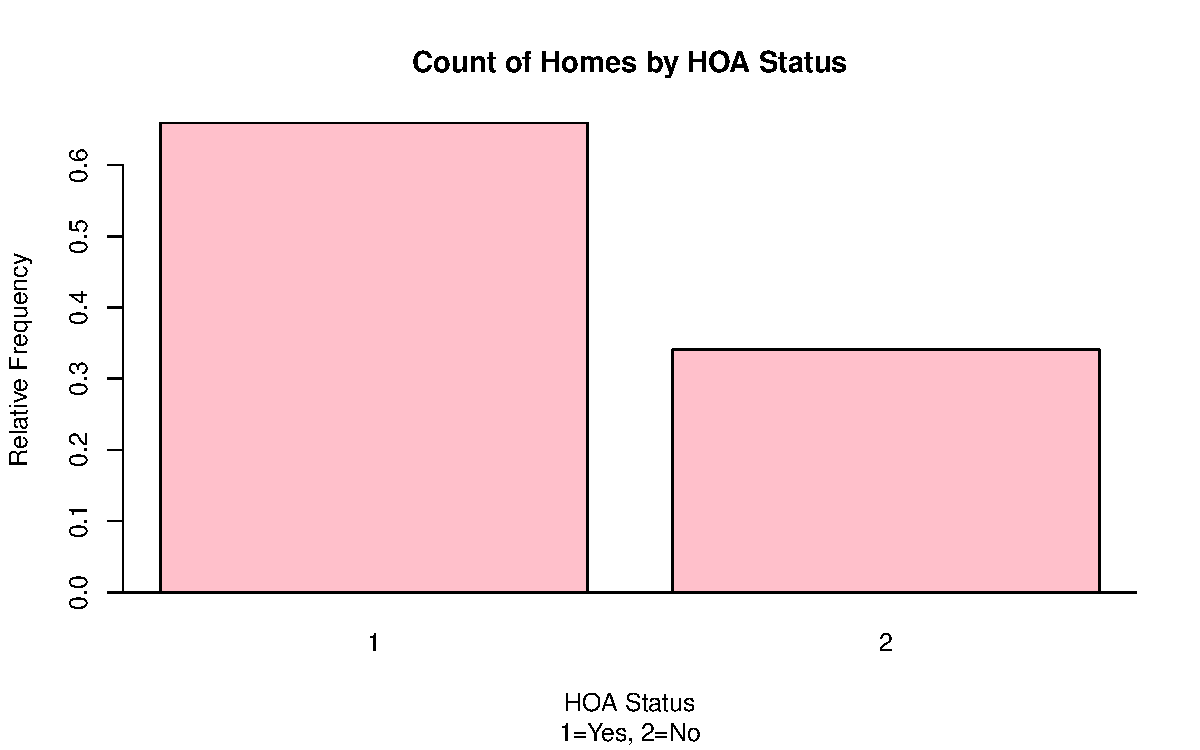
\includegraphics{exam1-007}

\begin{center} HOA Status of the Sample \end{center}
\begin{table}[h]
\begin{tabular}{ll}
HOA Status & Frequency \\
Yes        & 0.659176  \\
No         & 0.340824 
\end{tabular}
\end{table}


There seems to be almost twice as many homes in our sample that are a part of an HOA association as homes that are not a part of an HOA association. To be precise, 65.91 percent of homes in our sample are HOA homes and 34.08 percent of homes in our sample are non HOA homes. 


We should also look at these numbers in reference to different factors and compare breakdowns with homes that are part of an HOA and those that are not.


These graphs provide a side-by-side comparisons of households in HOAs and households not in HOAs, representing the relationships between these households' HOA statuses and multiple sustainability indicators. These graphs all utilize relative frequencies to compare proportionally between HOA households and non HOA households. As was illustrated by the previous graph, over 60 percent of the households in the sample are in an HOA while about 30 percent of households in the sample are not in an HOA. This will be important as we begin to analyze the homes by different factors. 


\newpage
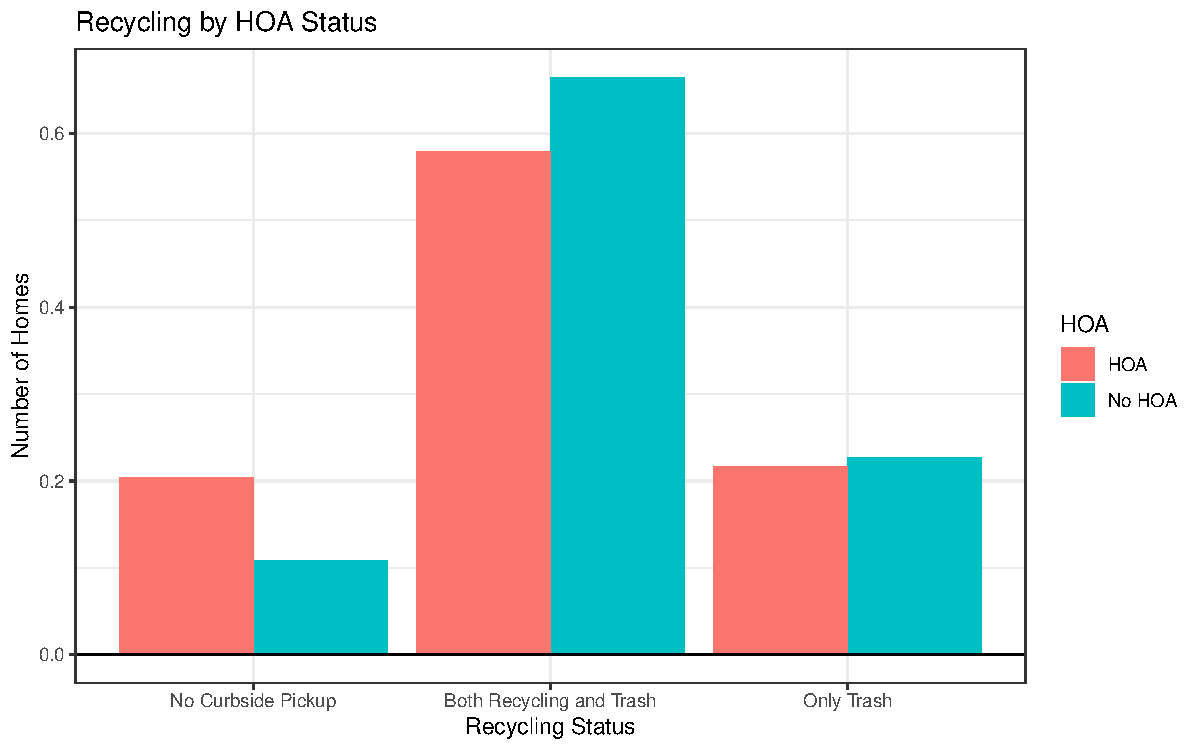
\includegraphics{exam1-008}
\newline
\begin{center}Recycling Status by HOA Status\end{center}
\begin{table}[h]
\begin{tabular}{lll}
HOA Status   & Recycle Status & Frequency      \\
HOA    & No Curbside Pickup       & 0.2035985 \\
HOA    & Both Recycling and Trash       & 0.5795455 \\
HOA    & Only Trash       & 0.2168561 \\
No HOA & No Curbside Pickup       & 0.1080586 \\
No HOA & Both Recycling and Trash       & 0.6648352 \\
No HOA & Only Trash       & 0.2271062
\end{tabular}
\end{table}


As we can see, regardless of HOA status homes the majority typically had both recycling and trash present. About 58 percent of HOA households and 66.5 percent of non HOA households had both trash and recycling pickup present. There were about the same proportion of homes that had only trash pickup for HOA and non HOA households (21.6 percent and 22.7 percent, respectively). About twice as many HOA households have no curbside pickup (20.4 percent) as non HOA households (10.8 percent). We can conclude from that that there is a higher proportion of non HOA homes to HOA homes that have either trash pickup or both recycling and trash pick up rather than no curbside pickup. This means that non HOA homes may be better for the environment compared to HOA homes in regards to recycling and waste management.


\newpage
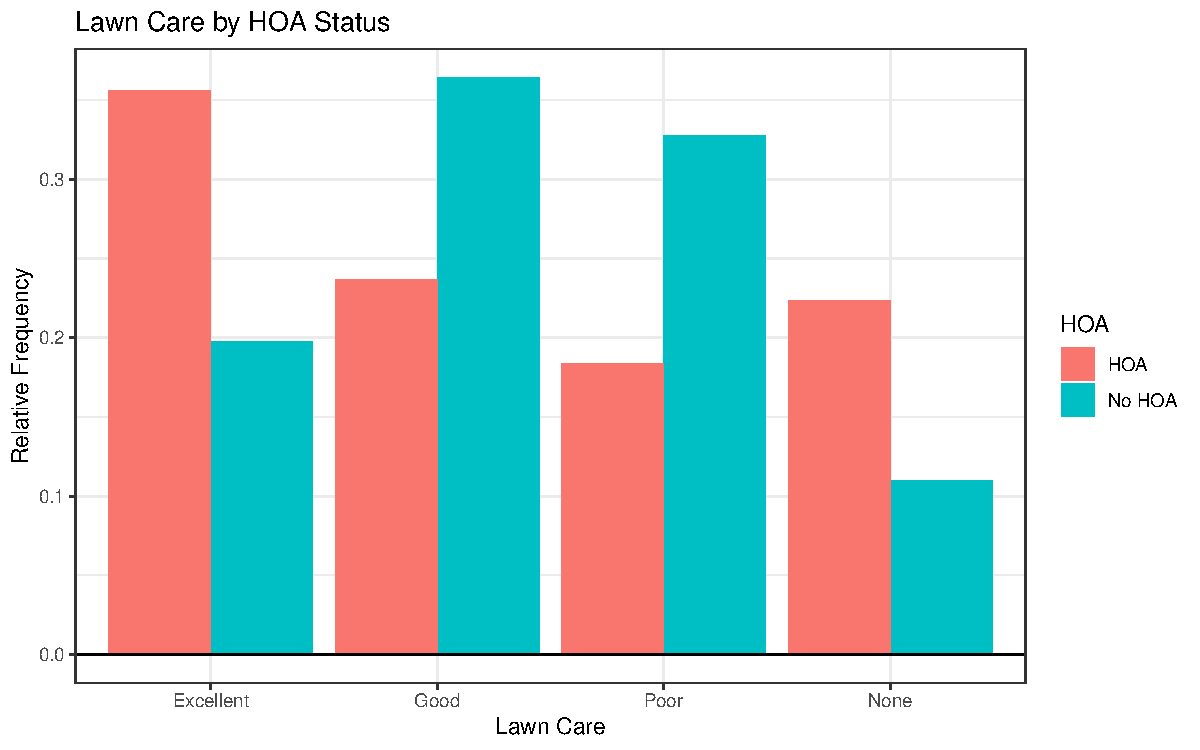
\includegraphics{exam1-009}

\begin{center} Lawn Care Status by HOA Status \end{center}
\begin{table}[h]
\begin{tabular}{lll}
HOA Status & Lawn Care Status & Frequency      \\
HOA    & Excellent         & 0.3560606 \\
HOA    & Good         & 0.2367424 \\
HOA    & Poor         & 0.1837121 \\
HOA    & None         & 0.2234848 \\
No HOA & Excellent         & 0.1978022 \\
No HOA & Good         & 0.3644689 \\
No HOA & Poor         & 0.3278388 \\
No HOA & None         & 0.1098901
\end{tabular}
\end{table}


As you can see from the charts above, households in HOAs had a higher percent of excellent lawn care (35.6 percent) than households without HOAs (19.8 percent). From this, we can infer that these households with HOAs typically use more chemical application than those without HOAs, which is worse for the environment. We also see that the highest percentage of homes not in an HOA have good (36.4 percent) or poor (32.8 percent) lawn care relative to homes in HOAs (23.7 percent and 18.4 percent, respectively). There is a pattern where lawn care for homes in HOAs fall on the full range of lawn care while homes not in HOAs fall in the good and poor types of lawn care. How much more damaging non HOA homes are compared to HOA homes in regards to lawn care is hard to say from the graph alone, but we can see from the table that more HOA households had excellent or good lawn care (about 59 percent) compared to non HOA households (about 56 percent). Again though, lawn care status alone may not be enough to determine if HOA households or non HOA households are better or worse for the environment. 

\newpage
\begin{table}[p]
\begin{tabular}{lll}
HOA Status & Trees & Frequency    \\
HOA        & 0     & 0.0643939394 \\
HOA        & 1     & 0.2632575758 \\
HOA        & 2     & 0.2159090909 \\
HOA        & 3     & 0.1562500000 \\
HOA        & 4     & 0.1079545455 \\
HOA        & 5     & 0.0672348485 \\
HOA        & 6     & 0.0501893939 \\
HOA        & 7     & 0.0255681818 \\
HOA        & 8     & 0.0160984848 \\
HOA        & 9     & 0.0094696970 \\
HOA        & 10    & 0.0056818182 \\
HOA        & 11    & 0.0037878788 \\
HOA        & 12    & 0.0028409091 \\
HOA        & 13    & 0.0056818182 \\
HOA        & 14    & 0.0018939394 \\
HOA        & 18    & 0.0018939394 \\
HOA        & 22    & 0.0009469697 \\
HOA        & 35    & 0.0009469697 \\
No HOA     & 0     & 0.0439560440 \\
No HOA     & 1     & 0.0952380952 \\
No HOA     & 2     & 0.1190476190 \\
No HOA     & 3     & 0.1355311355 \\
No HOA     & 4     & 0.0970695971 \\
No HOA     & 5     & 0.0989010989 \\
No HOA     & 6     & 0.0787545788 \\
No HOA     & 7     & 0.0512820513 \\
No HOA     & 8     & 0.0366300366 \\
No HOA     & 9     & 0.0641025641 \\
No HOA     & 10    & 0.0329670330 \\
No HOA     & 11    & 0.0293040293 \\
No HOA     & 12    & 0.0329670330 \\
No HOA     & 13    & 0.0183150183 \\
No HOA     & 14    & 0.0146520147 \\
No HOA     & 15    & 0.0109890110 \\
No HOA     & 16    & 0.0128205128 \\
No HOA     & 18    & 0.0018315018 \\
No HOA     & 19    & 0.0036630037 \\
No HOA     & 21    & 0.0036630037 \\
No HOA     & 22    & 0.0036630037 \\
No HOA     & 25    & 0.0018315018 \\
No HOA     & 28    & 0.0054945055 \\
No HOA     & 31    & 0.0036630037 \\
No HOA     & 35    & 0.0018315018 \\
No HOA     & 40    & 0.0018315018
\end{tabular}
\end{table}
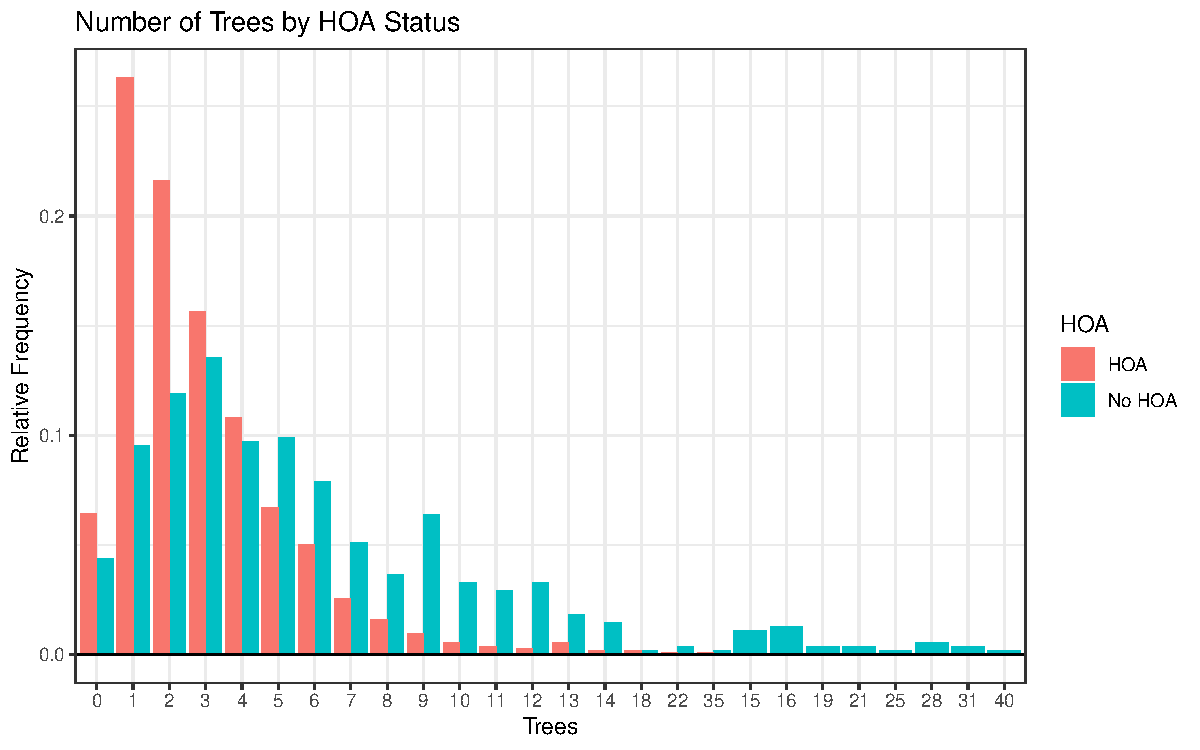
\includegraphics{exam1-010}

This figure illustrates the comparison between HOA homes and non HOA homes and the number of trees they have in their yard. It is important to note though that while most households in HOAs typically tend to have between 0 and 10 trees, it seems that households not in HOAs typically tend to have between 0 and 15 trees. In fact, about 62 percent of HOA homes have between 1 and 3 trees, where about half the proportion of non HOA homes (about 35 percent) have between 1 and 3 homes. The distribution of non HOA homes is less right skewed than the distribution of HOA homes, meaning a larger proportion of non HOA homes have more trees than HOA homes. From this, we can hypothesize that non HOA homes are more sustainable than HOA homes in the sense that non HOA homes have more trees planted than HOA homes, which is better for the environment.

\newpage
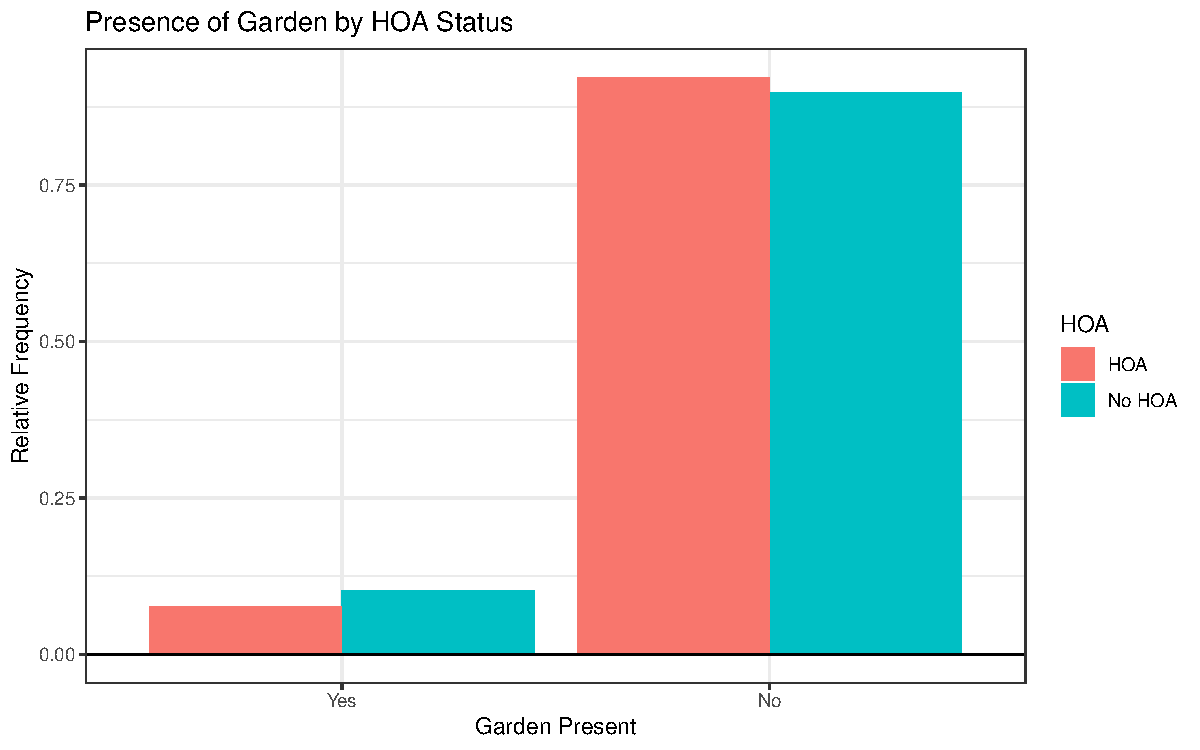
\includegraphics{exam1-011}

\begin{center} Garden Status by HOA Status \end{center}
\begin{table}[h]
\begin{tabular}{lll}
Garden & Frequency  & HOA Status \\
Yes     & 0.07765152 & HOA        \\
No    & 0.92234848 & HOA        \\
Yes     & 0.10256410 & No HOA     \\
No    & 0.89743590 & No HOA    
\end{tabular}
\end{table}


Households in and not in HOAs tend to follow a similar pattern when it comes to gardens. Both tend to not have gardens present in the front or back of their homes. 92.2 percent of HOA homes and 89.7 percent of non HOA homes did not have gardens in the yards. Therefore, in terms of garden status, HOA homes and non HOA homes have a similar, negative effect on the environment by not having gardens.
\newline

After examining sustainability factors at the household level, we can see that according to the number of trees in a home's yard and recycling status are clear indicators that non HOA homes are more sustainable than HOA homes. As a reminder, non HOA homes had more trees in their yard and better access to recycling and trash pickup compared to non HOA homes. Garden status and lawn care status gave results that did not clearly identify if HOA or non HOA homes were more sustainable. This is due to the fact that HOA and non HOA homes followed the same pattern of garden status. This indeterminate result also occurs because while HOA homes typically had more excellent lawn care than non HOA homes, they also had more lawns with no care than non HOA homes. Without knowing how many/much chemicals were used for the different lawn statuses of "excellent", "good", and "poor", it is hard to determine the environmental effects of homes in each category.
\newline


Now that we've seen the general count of observations with and without HOA, we can begin to examine multi-indicator sustainability analyses at the neighborhood level. We can do this by recreating the graphs that we previously created for each neighborhood. 
\newline

After looking at the data, we can split up neighborhoods by their HOA status.


Neighborhoods with HOAs are: Brownstone Crossing, Edgewood at Paris, Glastonbury Village, Half Mile Lake, Northcliff, Patridge Ridge


Neighborhoods without HOAs are: Buxton, Croftstone Acres, Fox Springs, Liberty Park, Timberlake, Windermere
\newline

If we were to proceed with this analysis, we would start by creating subsets of data for Neighborhoods that are HOA and non HOA, as we have already done for our previous analyses. From there, we could create 6 plots, 1 for each correlation relationship for the 4 variables of recycling, lawn care, garden, and trees. 
\newline
These 6 relationships would be recycling and lawn care, recycling and garden, recycling and trees, lawn care and garden, lawn care and trees, and garden and trees. These 6 plots could be two-way scatter plots fitted with regression lines to show the relationship between the two variables. It is important to note that since we don't know if the data was randomly collected, we cannot assume causality. These plots could be shown at the neighborhood level to compare HOA neighborhoods to non HOA neighborhoods. For each relationship, there are two plots that are differentiated by their regression lines. 
\newpage

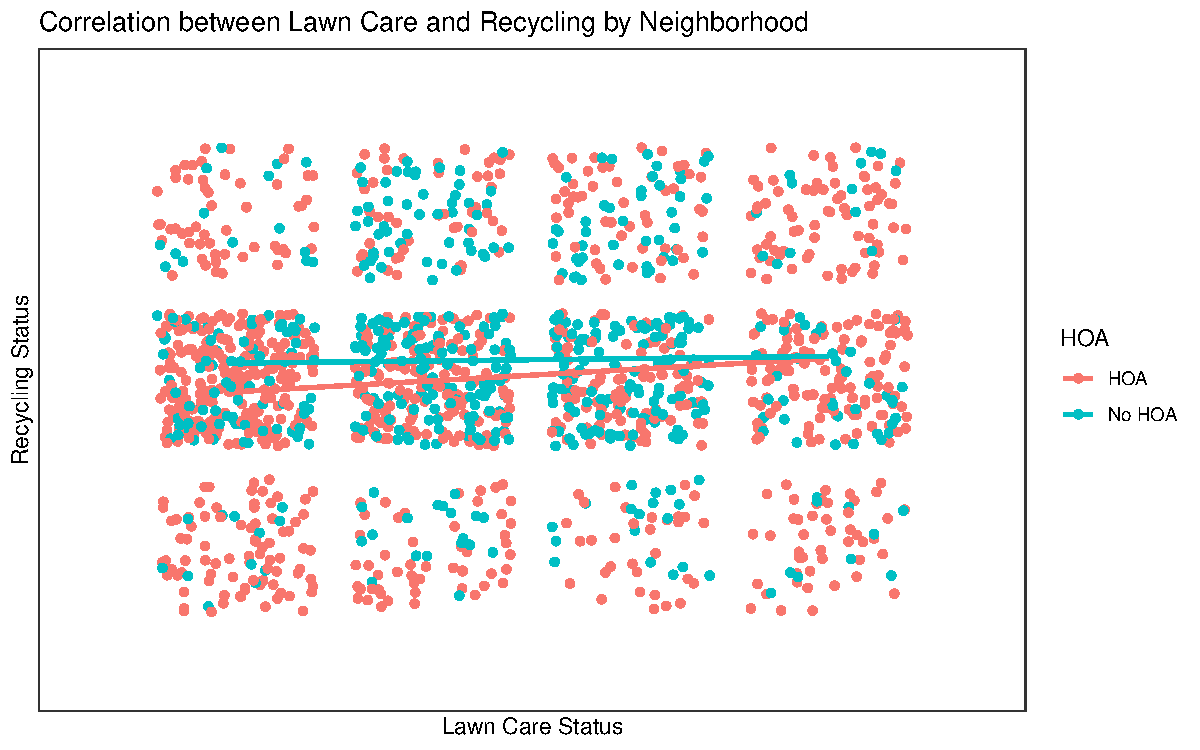
\includegraphics{exam1-012}
\newline
\begin{Schunk}
\begin{Sinput}
> rlcy<-table(dat.HOA.y$Recycle,dat.HOA.y$LawnCare)
> rlcy
\end{Sinput}
\begin{Soutput}
      1   2   3   4
  0  83  53  33  46
  1 238 149 106 119
  2  55  48  55  71
\end{Soutput}
\begin{Sinput}
> prop.table(rlcy)
\end{Sinput}
\begin{Soutput}
             1          2          3          4
  0 0.07859848 0.05018939 0.03125000 0.04356061
  1 0.22537879 0.14109848 0.10037879 0.11268939
  2 0.05208333 0.04545455 0.05208333 0.06723485
\end{Soutput}
\begin{Sinput}
> rlcn<-table(dat.HOA.n$Recycle,dat.HOA.n$LawnCare)
> rlcn
\end{Sinput}
\begin{Soutput}
      1   2   3   4
  0  12  19  18  10
  1  81 128 117  37
  2  15  52  44  13
\end{Soutput}
\begin{Sinput}
> prop.table(rlcn)
\end{Sinput}
\begin{Soutput}
             1          2          3          4
  0 0.02197802 0.03479853 0.03296703 0.01831502
  1 0.14835165 0.23443223 0.21428571 0.06776557
  2 0.02747253 0.09523810 0.08058608 0.02380952
\end{Soutput}
\end{Schunk}

\begin{center} Recycling Status by Lawn Care Status for HOA \end{center}
\begin{table}[H]
\begin{tabular}{lllll}
                           & None       & Poor       & Good       & Excellent  \\
No Trash Pickup            & 0.07859848 & 0.05018939 & 0.03125000 & 0.04356061 \\
Trash and Recycling Pickup & 0.22537879 & 0.14109848 & 0.10037879 & 0.11268939 \\
Trash Pickup Only          & 0.05208333 & 0.04545455 & 0.05208333 & 0.06723485
\end{tabular}
\end{table}

\begin{center} Recycling Status by Lawn Care Status for non HOA \end{center}
\begin{table}[H]
\begin{tabular}{lllll}
                           & None       & Poor       & Good       & Excellent  \\
No Trash Pickup            & 0.02197802 & 0.03479853 & 0.03296703 & 0.01831502 \\
Trash and Recycling Pickup & 0.14835165 & 0.23443223 & 0.21428571 & 0.06776557 \\
Trash Pickup Only          & 0.02747253 & 0.09523810 & 0.08058608 & 0.02380952
\end{tabular}
\end{table}

As we can see from the graph above, HOA neighborhoods tend to trend upwards more while non HOA neighborhoods tend to trend upwards and downwards. An upward trend indicates that as lawn care status improves (increasing chemical use), recycling and/or trash pickup becomes more likely for the neighborhood. A downward trend signals that as lawncare status improves, recycling and/or trash pickup becomes less likely for the neighborhood. This means that HOA neighborhoods may net out in terms of environmental sustainability. As lawn care status improves, meaning more chemicals are used on lawns which is bad for the environment, access to curbside pickup of trash and recycling becomes more likely which is good for the environment. Non HOA neighborhoods are have almost no relationship to lawncare status in this case. It is important to note that for some HOA neighborhoods, recycling status of no curbside pick had no relationship with lawn care status.

The tables can provide more insight into what exactly is going on in the relationship. About 60 percent of non HOA households have both Trash and Recycling Pickup and none, poor, or good lawn care. About 46 percent of HOA households have both Trash and Recycling Pickup and none, poor, or good lawn care. This is important because it shoes that non HOA neighborhoods have a larger proportion of their homes following good sustainability trends compared to HOA neighborhoods. 
\newpage

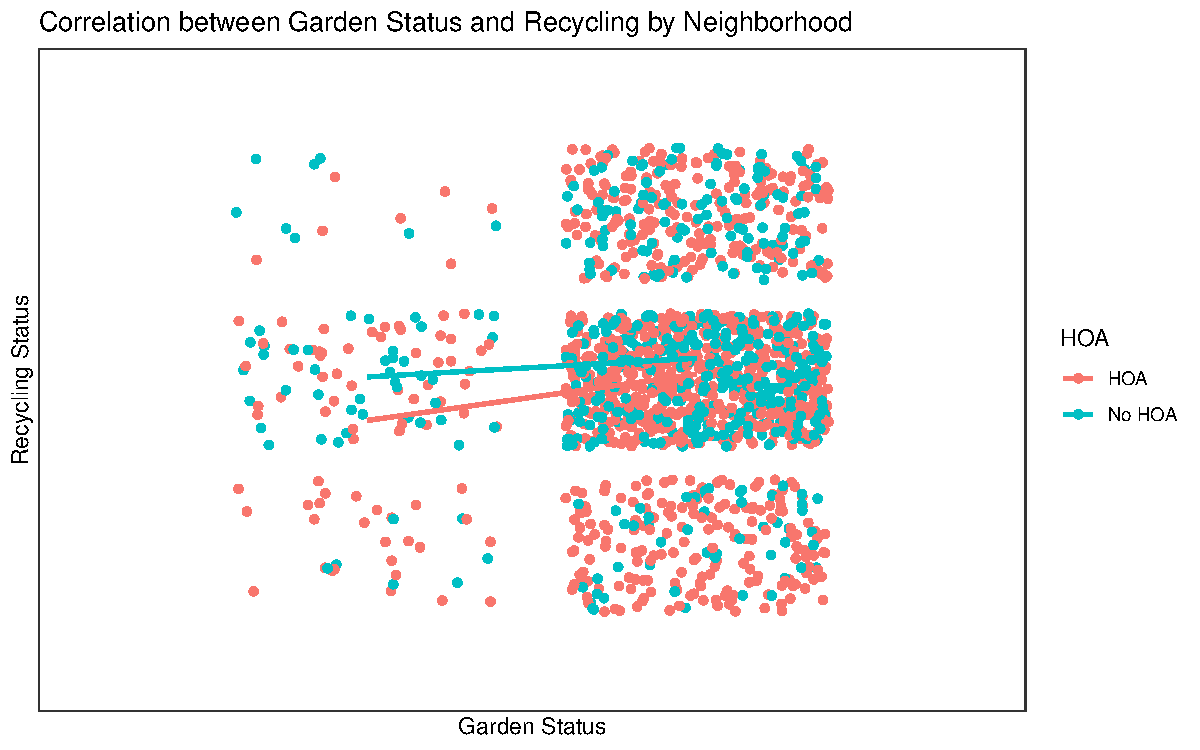
\includegraphics{exam1-014}
\newline
\begin{Schunk}
\begin{Sinput}
> rgy<-table(dat.HOA.y$Recycle,dat.HOA.y$Garden)
> rgy
> prop.table(rgy)
> rgn<-table(dat.HOA.n$Recycle,dat.HOA.n$Garden)
> rgn
> prop.table(rgn)
\end{Sinput}
\end{Schunk}

\begin{center} Recycling Status by Garden Status for HOA \end{center}
\begin{table}[H]
\begin{tabular}{lll}
                           & Yes         & No          \\
No Trash Pickup            & 0.025568182 & 0.178030303 \\
Trash and Recycling Pickup & 0.045454545 & 0.534090909 \\
Trash Pickup Only          & 0.006628788 & 0.210227273
\end{tabular}
\end{table}

\begin{center} Recycling Status by Lawn Care Status for non HOA \end{center}
\begin{table}[H]
\begin{tabular}{lll}
                           & Yes        & No         \\
No Trash Pickup            & 0.01282051 & 0.09523810 \\
Trash and Recycling Pickup & 0.07509158 & 0.58974359 \\
Trash Pickup Only          & 0.01465201 & 0.21245421
\end{tabular}
\end{table}

Examining the relationship between garden status and recycling status for HOA and non HOA neighborhoods, we can see that both kinds of neighborhoods following a similar trend. Neighborhoods with no gardens are more likely to have trash and/or recycling pickup. It is important to note that recycling status of no curbside pickup had no effect on some HOA neighborhoods' garden outcome. As we can see, overall HOA neighborhoods and non HOA neighborhoods had positive relationships between garden status and recycling status. This means that as the likelihood of gardens increased, recycling and/or trash pick up likelihood also increased. It is important to keep in mind though that HOA and non HOA households followed the same general trend of having no garden, so these graphs are not necessarily telling for differentiating between HOA and non HOA neighborhoods.

Examining the tables, we see that about 59 percent of non HOA homes had trash and recycling pickup and did not have a garden compared to 53 percent of HOA homes. After looking at the work that the researchers have done so far, it is unclear whether having a garden is sustainable or not. However, we can conclude from our other data and relationships that we've examined so far that non HOA homes typically tend to have more sustainable practices. We can therefore hypothesize that gardens may indicate bad sustainability, although their effects are probably small. Especially since gardens can be organic or not, contain different kinds of plants that are better or worse for soil and can be watered at different frequencies, their net effects are probably hard to determine from visuals alone. 

\newpage

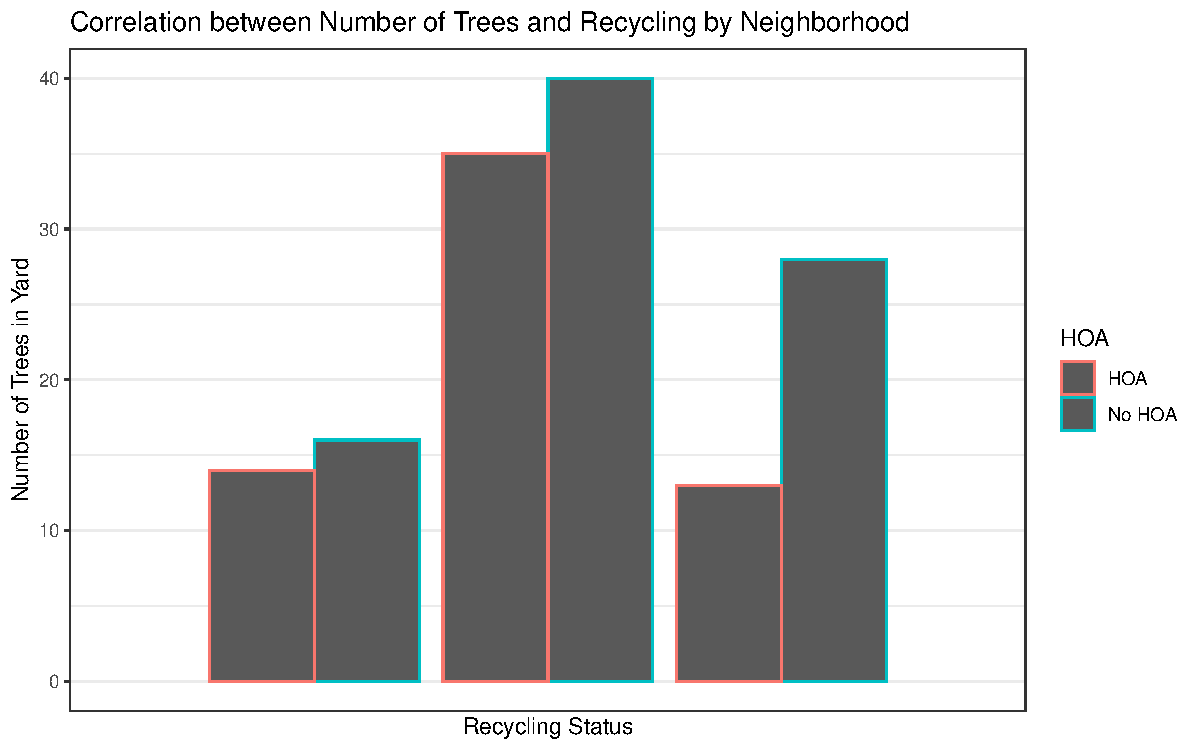
\includegraphics{exam1-016}
\newline
This graph illustrates that recycling and trash pickup is correlated with more trees for both HOA and non HOA neighborhoods, although non HOA neighborhoods have more trees generally. Not only that but there is a stronger relationship between trash pickup only and number of trees for non HOA households than HOA households. From this graph, we can posit that non HOA neighborhoods may be more sustainable than HOA neighborhoods because they have greater numbers of trees and instances of recycling and trash pickup or trash pickup only. 

\newpage

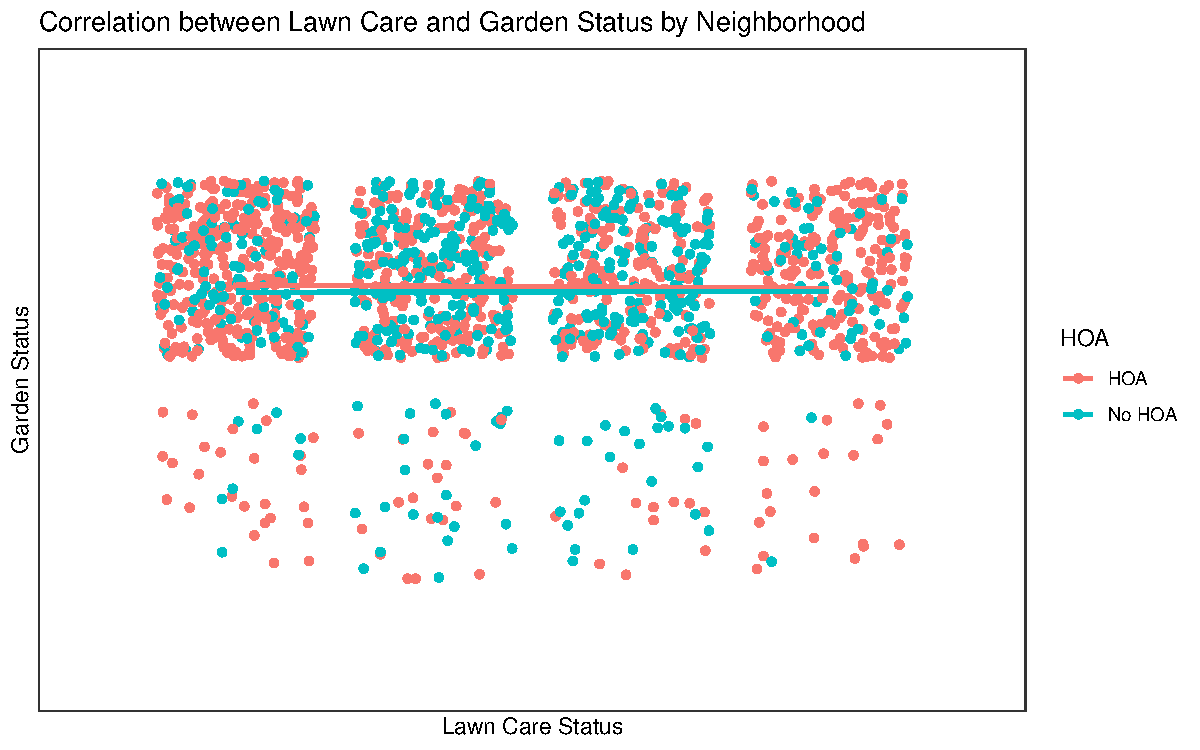
\includegraphics{exam1-017}

\begin{Schunk}
\begin{Sinput}
> lcgy<-table(dat.HOA.y$LawnCare,dat.HOA.y$Garden)
> lcgy
> prop.table(lcgy)
> lcgn<-table(dat.HOA.n$LawnCare,dat.HOA.n$Garden)
> lcgn
> prop.table(lcgn)
\end{Sinput}
\end{Schunk}

\begin{center} Lawn Care Status by Garden Status for HOA \end{center}
\begin{table}[H]
\begin{tabular}{lll}
          & Yes        & No         \\
None      & 0.02462121 & 0.33143939 \\
Poor      & 0.01988636 & 0.21685606 \\
Good      & 0.01325758 & 0.17045455 \\
Excellent & 0.01988636 & 0.20359848
\end{tabular}
\end{table}

\begin{center} Lawn Care Status by Garden Status for non HOA \end{center}
\begin{table}[H]
\begin{tabular}{lll}
          & Yes         & No          \\
None      & 0.014652015 & 0.183150183 \\
Poor      & 0.042124542 & 0.322344322 \\
Good      & 0.042124542 & 0.285714286 \\
Excellent & 0.003663004 & 0.106227106
\end{tabular}
\end{table}

From the graph, it is clear that there is little relationship between lawn care status and garden status due to the horizontal regression line. HOA neighborhoods and non HOA neighborhoods have a very slightly negative relationship between increasing lawn care status and increasing the likelihood of having a garden. Determining whether HOA or non HOA neighborhoods are more sustainable is hard to say in this case.

The tables show us that 55 percent of non HOA neighborhoods had no or poor lawn care while 58 percent of HOA neighborhoods had no or poor lawn care. These statistics alone may not be enough to show that one neighborhood is more sustainable than the other for this relationship. We see that about 10.6 percent of non HOA neighborhoods had excellent lawn care while about 22 percent of HOA neighborhoods had excellent lawn care. This indicates more that HOA neighborhoods may be less sustainable than non HOA neighborhoods because they use more chemicals for their lawn care. Again, since both HOA and non HOA neighborhoods have gardens around the same proportion, it is hard to compare these neighborhoods looking at both gardens status and lawn care status.
\newpage


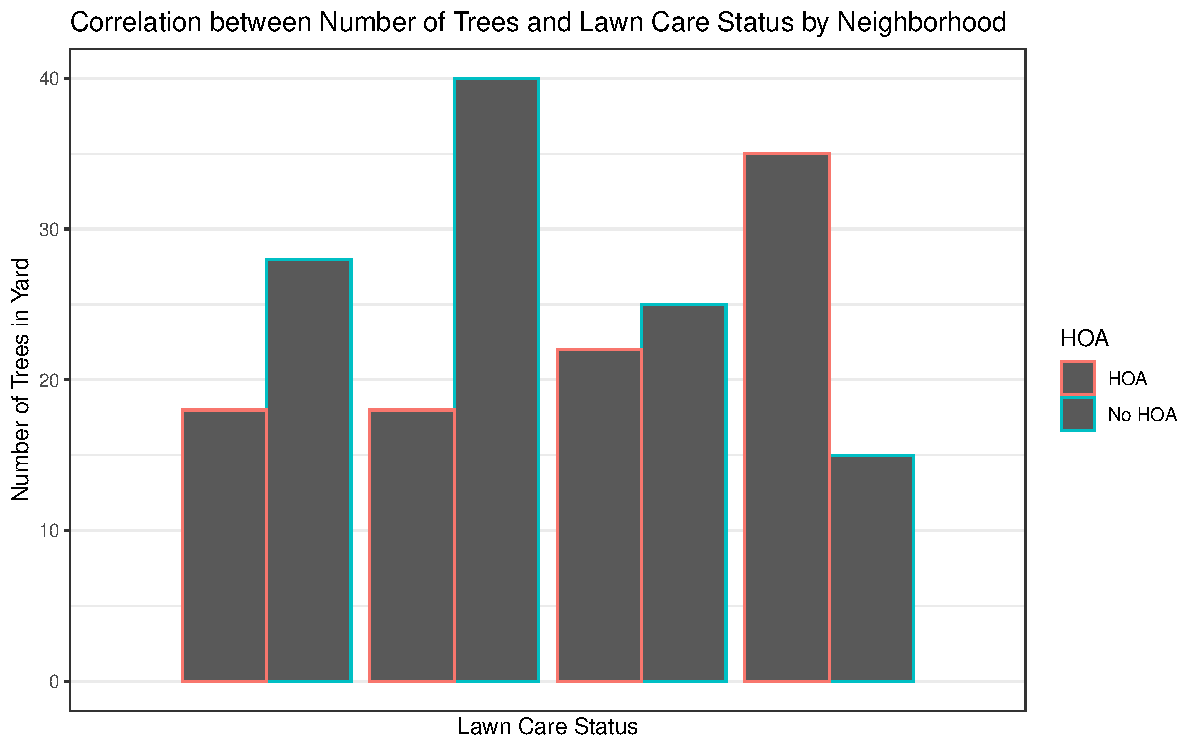
\includegraphics{exam1-019}
\newline
The graph above illustrates that non HOA neighborhoods are more sustainable than HOA neighborhoods because non HOA homes are more likely to have more trees and less lawn care compared to HOA neighborhoods. As we can see, the two kinds of neighborhoods follow different patterns. Non HOA neighborhoods follow a right skew pattern, where most observations have a lot of trees and little lawn care and then decrease the amount of trees they have as they increase their lawn care. HOA neighborhoods follow an increasing exponential pattern where none and poor lawn care statuses have fewer trees and as lawn care improves, the amount of trees seen on the property increases.
\newpage

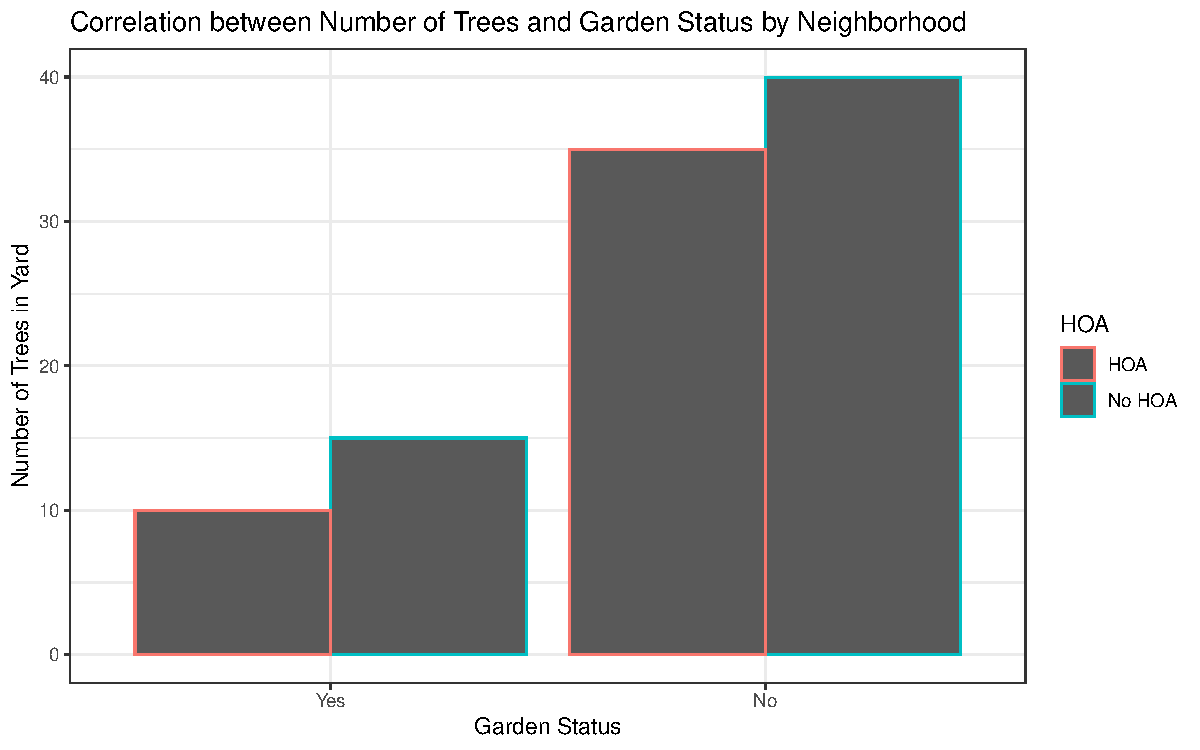
\includegraphics{exam1-020}
\newline
The graph above illustrates that regardless of garden status, non HOA neighborhoods have more trees than HOA neighborhoods. This important because as we discussed previously, garden status can be ambiguous when trying to determine if neighborhoods are more or less sustainable. However, having more trees is more sustainable. If non HOA neighborhoods have more trees regardless of garden status, then they can be seen as more sustainable than HOA neighborhoods.
\newline
Overall, we can see that non HOA neighborhoods are more sustainable than HOA neighborhoods. While some factors such as gardens may be ambiguous in terms of their sustainability, our analysis shows that non HOA neighborhoods have more trees, less lawn care, and more trash and recycling pickup options than HOA homes. Our sample had more HOA observations than non HOA observations, so we compared these variables using relative frequency for comparing HOA statuses to the four variables of lawn care, recycling, garden status, and trees, as well as illustrating relative frequency through tables for discrete vs. discrete variables and graphs for discrete vs. continuous variables. This paper encourages future researchers to look into the sustainability of gardens and what specific factors can be used to tell what gardens may or may not be sustainable. This research is important for potential homebuyers looking to purchase a sustainable home as well as those who are environmentally conscious and may or may not live in an HOA neighborhood.

\newpage
%attach bibliography and end document.
\bibliography{bib}
\end{document}
